\section{Mechanik}
\label{sec:Mechanik}

Damit die Maschine auch benutzt werden kann, wurde eine Mechanik entwickelt, welche aus folgenden Komponenten besteht: 

\begin{itemize}
\item Rahmen (Grundgerüst)
\item Getränkeschlitten 
\item Verkleidung
\item Unterbringung der Elektronik
\item Kühlbox
\end{itemize}

Nach dem alle Komponenten bekannt waren, wurde dabei vor der Bauphase ein Dreidimensionales Modell mittels des Windows Programm \flqq 3D Builder\frqq~gezeichnet, welches in Abbildung \ref{fig:3DModell} zu sehen ist. 

\begin{figure}[H]
	\centering
	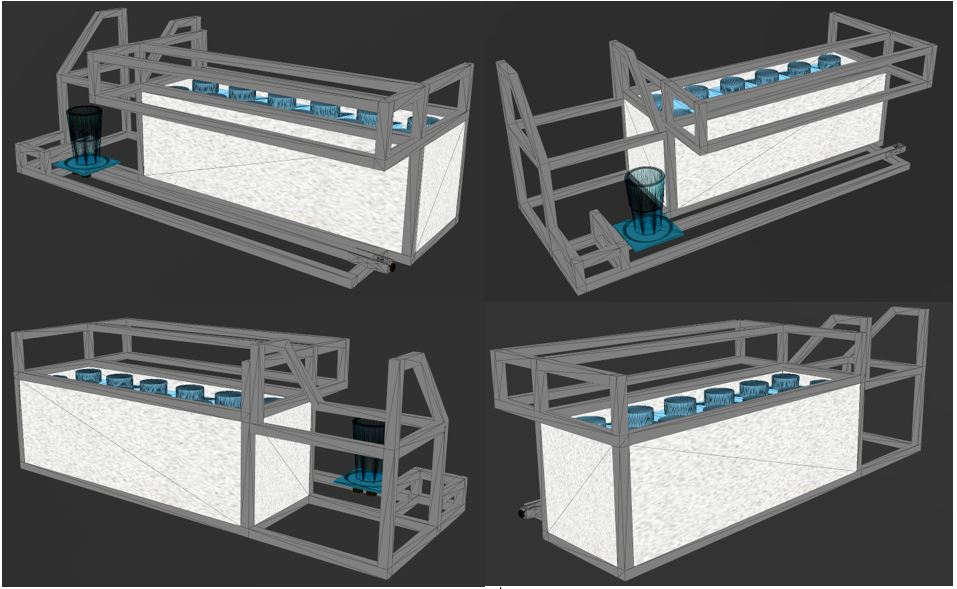
\includegraphics[width=0.8\textwidth]{graphics/3DModell}
	\caption{3D-Modell des Partymixers}.
	\label{fig:3DModell}
\end{figure}

